\documentclass{article}

\usepackage{graphicx}
\usepackage{tabularx}

\title{\Huge Compte Rendu Hashtable}
\date{19-02-2024}
\author{Wilhem Blondel (21212622) et Alexandre Genin (21131809)}

\begin{document}
    \pagenumbering{gobble}
    \maketitle
    \newpage
    \pagenumbering{arabic}

    \section{Question 3.1 et 3.2}

    Pour effectuer la comparaison de temps de calcul entre la table de hachage, nous avons créer
    le fichier \texttt{comparaison.c} qui effectue 100 recherches consécutives 
    dans la liste chaînée, puis dans la table hachage de taille donnée. 
    \newline
    Les deux structures ont chargés l'intégralité de la bibliothèque de 10000 livres,
    l'élément recherché était le même à test et avait une position éloigné 
    d'environ 7700 blocs de la tête de liste.
    \newline
    Les résultats observées sont les suivants:

    \begin{table}[h]
        \centering
            \begin{tabularx}{\textwidth}{ |*{5}{>{\centering\arraybackslash}X|} }
                \hline
                Type de recherche& Liste chaînée & Hastable (500 clés)  & Hashtable (50 clés) & Hashtable \newline (5 clés)\\
                \hline
                Numéro connu & 0.014844 ms & 0.237934 ms & 0.205067 ms &  0.157843 ms\\
                Numéro inconnu & 0.088723 ms & 0.510378 ms & 0.491641 ms & 0.343747 ms\\
                \hline
                Titre connu & 0.020914 ms & 0.299899 ms & 0.284141 ms & 0.227464 ms\\
                Titre inconnu & 0.098122 ms & 0.494885 ms & 0.500609 ms & 0.325849 ms \\
                \hline
                Auteur connu & 0.091525 ms & 0.000130 ms & 0.005319 ms & 0.036859 ms \\
                Auteur inconnu & 0.092567 ms & 0.000166 ms & 0.005531 ms &  0.037656 ms \\
                \hline
            \end{tabularx}
        \caption{Temps de recherche d'une même donnée sur différentes structures}
        \label{tab:hashVSLC}
    \end{table}

    On peut observer ici que la taille de la Hashtable influe en partie sur la vitesse de recherche.
    \newline
    Lorsque l'on recherche selon l'auteur, une table de hachage avec une taille plus importante
    est plus efficace qu'une table ayant une taille plus faible. Ce résultat n'est pas surprenant
    car une table avec une taille plus importante minimise les collisions.
    \newline
    Remarquons néanmoins que peu importe la taille de la table de hachage, le temps de recherche
    est significativement moins important que dans une liste chaînée quand il s'agit de chercher l'auteur
    \newline
    En revanche observons que le temps de recherche est plus important dans une table de hachage que
    dans une liste chaînée lorsque l'on recherche par numéro ou par titre. Ceci est dû au fait que la
    clé de la table ne dépend pas de ces informations. Ce résultat était effectivemment prévisible.
    \newline
    Lorsque l'on cherche un livre par son numéro, on cherche d'abord dans une certaine case du tableau,
    et on parcourt la liste chaînée associée à cette case. Il faut donc le temps de sauter d'une case
    du tableau à l'autre, et le temps de parcours d'une liste chaînée.
    \newline
    On observe donc de façon logique que plus la table de hachage est petite, plus la recherche à partir
    d'un numéro ou d'un titre est moindre
    
    \newpage
    \section{Question 3.3 et 3.4}
    Pour effectuer cette comparaison, nous avons préparé un nouveau code: 
    \texttt{courbes.c}
    \newline
    Ce code nous permet d'exécuter la fonction de recherche de doublons sur 
    différentes tailles de bibliothèque, et de comparer le temps d'exécution
    entre une liste chaînée et une table de hachage.
    \newline
    Au début, nous avons décidé d'adapter la taille du tableau de hachage en
    fonction du nombre de livres qu'il contient. (Pour $n$ livres sa taille
    était de $\frac{n}{2}$). 
    \newline
    Les courbes étaient les suivantes:
    \begin{figure}[h]
        \centering
        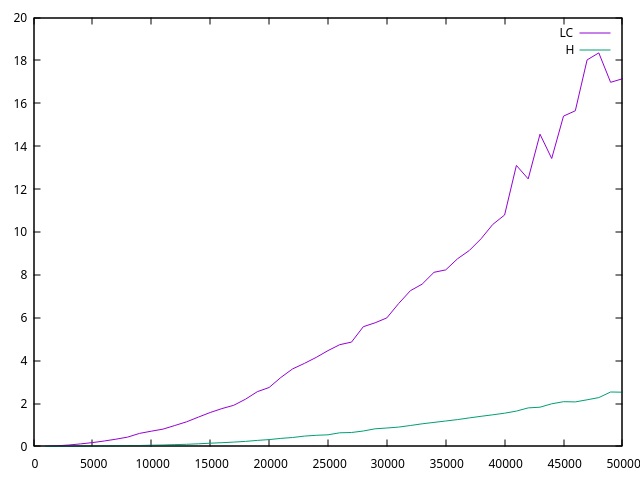
\includegraphics[width=0.5\textwidth]{graph.png}
        \caption{Temps de calcul entre une liste chaînée et hashtable de 20 clés}
        \label{fig:hash20}
    \end{figure}


        
\end{document}
